\section{Глубокое обучение} \label{ch1:dl}

Глубокое обучение (Deep Learning, \hyperref[acr:dl]{DL}) - подраздел машинного обучения, с применением которого в настоящее время достигаются выдающиеся результаты во многих областях, в том числе в распознавании изображений, компьютерном зрении, распознавании речи и обработке естесственных языков. Глубокое обучение как бы имитирует биологический мозг, обрабатывает информацию с помощью искусственных нейронных сетей.

Идея симуляции работы нейронов мозга человека зародилась десятилетия назад. Тем не менее, прорыв произошёл в последние годы, когда стали доступны большие наборы данных и вычислительные мощности \cite{10.1145/2771283}. Теперь можно строить модели с большим количеством слоёв искусственных нейронов, чем когда-либо прежде. Сети достигают исключительной производительности в области распознавания изображений и речи при значительном увеличении глубины. Считается, что глубокое обучение является одним из наиболее перспективных подходов для решения текущих задач ИИ.

\subsection{Искусственная нейронная сеть}

Мозг человека и животных - чрезвычайно сложный орган, который до сих пор до конца не изучен. Тем не менее, некоторые аспекты его структуры и функции были расшифрованы. Фундаментальным рабочим элементом в мозге является нейрон. Многочисленные нейроны связаны между собой сложным образом, что даёт возможность запоминания, мышления и принятия решений.

Хотя нейроны сложны и функционируют разными способами, все они имеют некоторые базовые компоненты такие как: ядро, дендриты, аксон и синапсы. Дендриты действуют как входные каналы, через которые нейроны получают информацию от синапсов других нейронов. Затем ядро обрабатывает эти сигналы и превращает в вывод, который затем отправляется в другие нейроны. Связь этих компонентов играет роль линии передачи в нейронных сетях.

Хоть \hyperref[acr:ann]{ИНС} и не так сложны, как человеческий мозг, они имитируют базовую структуру, которая включает входные, выходные слои, а также, обычно, скрытые слои. В каждом слое есть искусственные нейроны. Нейроны в одном слое обычно связаны с каждым нейроном в следующем слое. Они передают числовые сигналы через соединения с другими нейронами, примерно, как это происходит в биологической нейронной сети \cite{296402}.

Поскольку выходные сигналы нейронов ИНС представляются в виде вещественных чисел, выход обычно сравнивается с порогом. Только в том случае, если порог превышен, нейрон передаёт сигнал следующим подключённым нейронам.

\begin{figure}[ht!]
    \center
    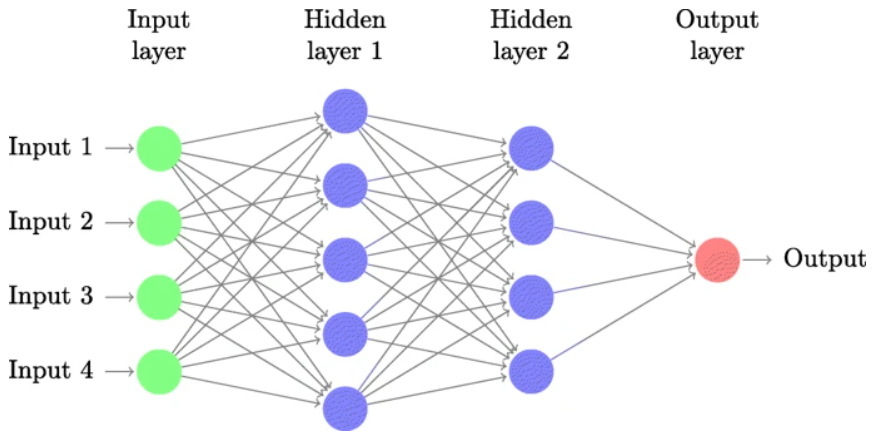
\includegraphics [scale=0.60] {my_folder/images/ch1/ANN.png}
    \caption{Базовая структура ИНС. ИНС обычно состоит из входного и выходного слоёв, а также пары скрытых слоёв. Основано на \cite{Khajanchi2003ArtificialNN} \cite{mitchell1997machine}}
    \label{fig:ch1-ANN}
\end{figure}

Связи между нейронами параметризованы весами, которые обновляются во время обучения, чтобы отрегулировать мощность сигналов, проходящих через сеть [24]; \firef{fig:ch1-ANN} показывает базовую структуру ИНС.

\subsection{Глубокая нейронная сеть}

Как уже упоминалось выше, концепция нейронной сети не нова.

На ранних этапах из-за ограничений вычислительной мощности, нейронные сети имели очень малую глубину. Обычно они содержали только входной, выходной слои и пару скрытых слоёв. Кроме того, количество нейронов в каждом слое также было ограничено. Глубокие нейронные сети не находили практического применения до последних лет, когда стали доступны огромные вычислительные мощности и большие объёмы данных.

Глубокие нейронные сети с несколькими слоями хороши для извлечения скрытых свойств \cite{7344858}. Каждый слой решает свою собственную задачу. Узлы в каждом слое учатся на конкретных наборах свойств, которые приходят из предыдущего слоя. Теоретически, чем глубже нейронная сеть, тем более сложны и абстрактны особенности, которые она может распознать, поскольку каждый нейрон агрегирует выводы из нейронов предыдущего слоя \cite{bengio2012representation}. Например, в задаче распознавания изображений вход представляет собой матрицу пикселей. Первый слой извлекает начальные объекты, такие как рёбра из пикселей, затем следующий слой кодирует расположение краёв и следующий слой распознаёт глаза, рот, уши, ноги, крылья, хвост и т.д. Наконец, последний слой распознаёт на изображении кошку, собаку или птицу. Таким образом, глубокие нейронные сети не нуждаются во вмешательстве людей, а сами изучают иерархию объектов.

С математической точки зрения нейронная сеть определяет функцию ${y = f(x; \theta)}$. Она описывает соответствие входных данных ${x}$ выходным ${y}$, где ${y}$ --- это категория в задаче классификации или выходное значение в задачах регрессии. Тренировка модели с использованием набора данных ведёт к вычислению параметра {$\theta$}.

После завершения обучения предполагается, что нейронная сеть аппроксимирует целевую функцию ${f^*}$ \cite{Goodfellow-et-al-2016}. Правильно обученная ИНС может лучше соответствовать набору данных, а также делает прогноз, учитывая неочевидные зависимости от данных.

Глубокие нейронные сети могут быть реализованы по-разному в зависимости от конкретных практических задач. Например, свёрточные нейронные сети специализируются на компьютерном зрении, а рекуррентные нейронных сети лучше подходят для обработки естественного языка.

Функцию отображения ${f(x)}$ можно рассматривать как цепочку из многих связанных функций в виде  ${f(x) = f^{(n)}(f^{(n-1)}(...f^{(2)}(f^{(1)}(x))))}$; ${n}$ связанных функций соответствуют глубине ИНС. Функция стоимости определяется на основе сравнения вывода ${y}$ из ${f(x)}$ с целевым значением ${t}$ из тренировочного набора данных. Цель обучения нейронной сети состоит в том, чтобы приблизить ${f(x)}$ функцей, минимизирующей функцию стоимости. Минимизация функции стоимости является задачей оптимизации, и для этого часто используют алгоритм {\itshape градиентного спуска}. В {\itshape обратном распространении} (backpropagation) градиент используется для итеративного обновления нейронной сети во время обучения. Оптимизатор решает, какие параметры и как должны быть обновлены, а {\itshape скорость обучения} (learning rate) задаёт размер шага, на который параметр обновляется на каждой итерации.
